\documentclass{beamer}
\usetheme{AnnArbor}
\usecolortheme{beaver}
\usepackage{setspace}
\usepackage{color}
\usepackage{listings}

% \usepackage{beamerthemesplit} // Activate for custom appearance

\title{Using Django Rest Framework}
\subtitle{To Simplify Your App}
\author{Ed Henderson}
\date{\today}

\begin{document}

\lstset{breakatwhitespace=true,
basicstyle=\ttfamily\scriptsize,
language=python,
backgroundcolor=\color{gray},
numbers=left, numberstyle=\tiny, stepnumber=1, numbersep=5pt,
columns=fullflexible,
keepspaces=true,
keywordstyle=\color{blue}\bfseries,
%breaklines=true,
tabsize=1, 
showstringspaces=false,
extendedchars=true}

\frame{\titlepage}

%\section[Outline]{}
\frame{\tableofcontents}

\section{What's in the box}
\begin{frame}

  \frametitle{Core Features}

Everything you need to build a REST API

  \begin{itemize}
  \item Serializers
  \item Renderers and Parsers
  \item Views, Viewsets
  \item Routers
  \item Authentication and Permissions
  \item Throttling, Filtering, Pagination, Versioning
  \end{itemize}
\end{frame}

\section{Serializers}
\begin{frame}[fragile]

  \frametitle{Serializers}

  \begin{itemize}
  \item Convert your data into Python native datatypes.
  \item Used to convert a DB Model (or Models) into native types
  \item Works with Foreign Keys, and arrays of objects. 
  \item Deserialize data also.
  \end{itemize}
  
\end{frame}

\begin{frame}[fragile]

  \frametitle{Example: Serialize an Object}

  \begin{itemize}
  \item Basic Python Object, not a model
  \end{itemize}
  
  \begin{lstlisting}
class SomeObject(object):

    def __init__(self, charfield, floatfield, intfield, emailfield):
        self.charfield = charfield
        self.floatfield = floatfield
        self.intfield = intfield
        self.emailfield = emailfield

    def __str__(self):
        return "SomeObject:{} - {} - {} -{}".format(
            self.charfield, self.floatfield, self.intfield, self.emailfield
        )
    \end{lstlisting}

\end{frame}

\begin{frame}[fragile]

  \frametitle{Example: Simple Object Serializer}

\begin{itemize}
	\item Same format as Model and Form definitions
	\item Must provide explicit create and update methods
\end{itemize}
\begin{lstlisting}
        
class ObjectSerializer(serializers.Serializer):
    charfield = serializers.CharField(max_length=100)
    floatfield = serializers.FloatField()
    intfield = serializers.IntegerField()
    emailfield = serializers.EmailField()

    def create(self, validated_data):
        return SomeObject(**validated_data)

    def update(self, instance, validated_data):
        """
        Check each param, and update as needed on the instance..
        """
        # Update the instance
        return instance
    \end{lstlisting}

\end{frame}

\begin{frame}[fragile]

  \frametitle{Example: Simple Object Serializer - save}

\begin{itemize}
	\item create function used during save
	\item update function used during update
\end{itemize}

\begin{lstlisting}
# Save
        serializer = ObjectSerializer(data=data)
        serializer()
        obj = serializer.save()
        
# Update
        serializer = ObjectSerializer(instance, data=data)
        serializer()
        obj = serializer.save()        
\end{lstlisting}

\end{frame}

\begin{frame}[fragile]

  \frametitle{Serializer Fields and Validation}

\begin{itemize}
	\item Standard fields have basic validation
	\item Field types define basic validation
	\item Define read or write only fields
	\item Allow null fields, provide defaults, specify a field validator
	\item def validate() for object level validation
	\item Can create custom fields also
\end{itemize}


\end{frame}

\begin{frame}[fragile]

  \frametitle{Serializers can be nested}

\begin{itemize}
	\item Serializer class is a 'Field' type
	\item Handle complex hierarchies of objects
	\item Nested serializer could be a list of items
	\item create() and update() methods more complex
	
\end{itemize}

\begin{lstlisting}
class CommentSerializer(serializers.Serializer):
    user = UserSerializer(required=False)
    edits = EditItemSerializer(many=True)  # A nested list of 'edit' items.
    content = serializers.CharField(max_length=200)
    created = serializers.DateTimeField()
\end{lstlisting}

\end{frame}

% ----------------------------------------
\begin{frame}[fragile]

  \frametitle{Model Serializers}

\begin{itemize}
	\item Uses introspection to determine fields
	\item Creates model validators, i.e. "unique together"
	\item Creates default save and update methods
	\item Default behavior handles most situations
	
\end{itemize}

\begin{lstlisting}
class SomeModelSerializer(serializers.ModelSerializer):
    class Meta:
        model = SomeModel
        fields = (<list of fields>) # defaults to all fields
\end{lstlisting}

\end{frame}

% ----------------------------------------
\begin{frame}[fragile]

  \frametitle{Model Serializers: Extending}

\begin{itemize}
	\item Add additional fields to a serializer
	\item Fields can be based on a value, property or function
	\item Specify a different field type than the default
\end{itemize}

\begin{lstlisting}
class SomeModelSerializer(serializers.ModelSerializer):
    extra_field = serializers.CharField(source='get_extra_data', read_only=True)
    
    class Meta:
        model = SomeModel
        fields = (<list of fields>) # defaults to all fields
\end{lstlisting}

\end{frame}

% ----------------------------------------
\begin{frame}[fragile]

  \frametitle{Model Serializers: Relations}

\begin{itemize}
	\item Handling of Foreign Key, OneToOne, ManyToMany Fields
	\item Default is to list the ID as an integer
	\item Other choices
		\begin{itemize}
		\item StringRelatedField
		\item<2-> PrimaryKeyRelatedField (default)
		\item<3-> HyperlinkedRelatedField
		\item<4-> SlugRelatedField
		\item<5-> HyperlinkedIdentityField
		\item<6-> Nested  Relationship
		\end{itemize}
\end{itemize}

\begin{lstlisting}
tracks = serializers.StringRelatedField(many=True)
tracks = serializers.PrimaryKeyRelatedField(many=True, read_only=True)
tracks = serializers.HyperlinkedRelatedField(...)
tracks = serializers.SlugRelatedField(...)
tracks = TrackSerializer(many=True, read_only=True)
\end{lstlisting}

\end{frame}

% ----------------------------------------
\begin{frame}[fragile]

  \frametitle{Serializers: What did I skip?}

\begin{itemize}
	\item Take control of field mapping
	\item Specify some field type defaults: url, or choice fields
	\item Customization
	
\end{itemize}

\end{frame}

\section{Renderers and Parsers}
\begin{frame}[fragile]

  \frametitle{Renderers and Parsers}

  \begin{itemize}
  \item Serializers convert your object/model to/from Python native datatypes.
  	\begin{itemize}
		\item Lists
		\item Dictionaries
        		\item String, Float, Int
	\end{itemize}
  \item Renderers/Parsers convert to/from
  	\begin{itemize}
            	\item JSON
            	\item Template HTML
            	\item Static HTML
            	\item Browsable API
	\end{itemize}
  \end{itemize}
  
\end{frame}

\begin{frame}[fragile]

  \frametitle{Which renderer to use?}

  \begin{itemize}
  	\item Accept header 
            \begin{itemize}
            \item text/html
            \item application/json
            \end{itemize}
  	\item .format headers 
            \begin{itemize}
            \item .json
            \item .xml
            \end{itemize}
  	\item query parameters
            \begin{itemize}
            \item format=json
            \item format=xml
            \end{itemize}
  \end{itemize}
  
\end{frame}

\section{Views and Viewsets}
\begin{frame}[fragile]

  \frametitle{Generic Views}

  \begin{itemize}
  \item Just covering Class based views
  \item Views assembled from Mixins and a GenericAPIView
  \item GenericAPIView based on APIView 
  	\begin{itemize}
		\item Authentication, Throttling
		\item Content negotiation
		\item get\_queryset, get\_object
        		\item Serialization, filtering
		\item Pagination
	\end{itemize}
  \end{itemize}
  
\end{frame}

\begin{frame}[fragile]

  \frametitle{Mixins}

  \begin{itemize}
    	\item Used when assembling a working generic
	\item Can be used in your own views also
      	\item Add the core functions
		\begin{itemize}
    			\item create (CreateModelMixin)
    			\item list (ListModelMixin)
    			\item retrieve (RetrieveModelMixin)
            		\item update, partial\_update (UpdateModelMixin)
    			\item destroy (DestroyModelMixin)
    		\end{itemize}
  \end{itemize}
  
\end{frame}

\begin{frame}[fragile]

  \frametitle{REST method mapping}

  \begin{itemize}
  	\item 
      	\item get
		\begin{itemize}
    			\item list
    			\item retrieve
    		\end{itemize}
      	\item post
		\begin{itemize}
    			\item create
    		\end{itemize}
      	\item put
		\begin{itemize}
    			\item update
    		\end{itemize}
      	\item patch
		\begin{itemize}
    			\item partial\_update
    		\end{itemize}
      	\item delete
		\begin{itemize}
    			\item destroy
    		\end{itemize}
  \end{itemize}
  
\end{frame}

\begin{frame}[fragile]

  \frametitle{Mapping Views}

  \begin{itemize}
  	\item Too many of these view types to list 
	\item take a look in generics file
	\item Contains most of the combinations you will need
	\item Or, roll your own
  \end{itemize}
 
\begin{lstlisting}
class ListCreateAPIView(mixins.ListModelMixin,
                        mixins.CreateModelMixin,
                        GenericAPIView):
    """
    Concrete view for listing a queryset or creating a model instance.
    """
    def get(self, request, *args, **kwargs):
        return self.list(request, *args, **kwargs)

    def post(self, request, *args, **kwargs):
        return self.create(request, *args, **kwargs)

\end{lstlisting}
  
\end{frame}

\begin{frame}[fragile]

  \frametitle{ViewSets}

  \begin{itemize}
  	\item A Class based view with action methods
	\item create, retrieve, update, destroy, ...
	\item Manually mapped to a REST operation
	\item Or, dynamically mapped using routers.
	\item ModelViewSet provide the kitchen sink
  \end{itemize}
 
\begin{lstlisting}
class ModelViewSet(mixins.CreateModelMixin,
                   mixins.RetrieveModelMixin,
                   mixins.UpdateModelMixin,
                   mixins.DestroyModelMixin,
                   mixins.ListModelMixin,
                   GenericViewSet):
    """
    A viewset that provides default `create()`, `retrieve()`, `update()`,
    `partial_update()`, `destroy()` and `list()` actions.
    """
    pass

\end{lstlisting}
  
\end{frame}

\section{Routers and URLs}
\begin{frame}[fragile]

  \frametitle{URL Mapping}

	Now we have some shiny new views, but need to map them to a set of URLs
  \begin{itemize}
  \item list: '\^widget\/\$'
  \item retrieve: '\^widget\/\{pk\}\/'
  \item update: '\^widget\/\{pk\}\/'
  \item destroy: '\^widget\/\{pk\}\/'
  \item We need different operations for some of these URLs....
  \end{itemize}
  
\end{frame}

\begin{frame}[fragile]

  \frametitle{Routers}

  \begin{itemize}
  \item Use introspection to determine what action methods exist
  \item Builds the URLs for you, and maps the REST methods
  \item Define custom methods with \@list\_route and \@detail\_route
  \end{itemize}
  
  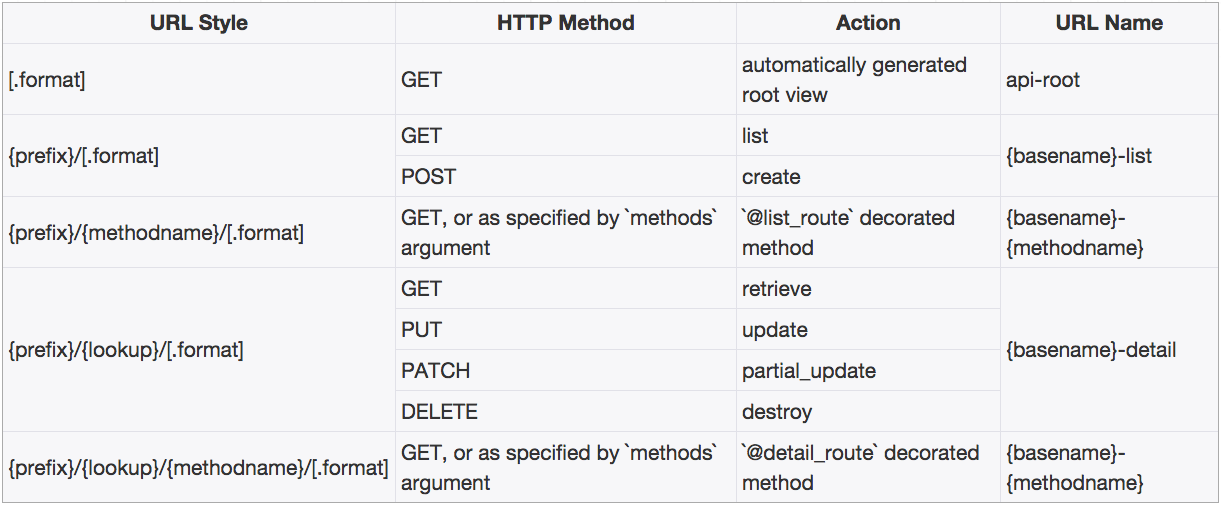
\includegraphics[width=0.99\textwidth]{images/drf_default_router.png}
  
\end{frame}

\section{Authentication and Permissions}
\begin{frame}[fragile]

  \frametitle{Authentication}

  \begin{itemize}
      \item Easily add Authentication requirements to any API point
            \begin{itemize}
                \item BasicAuth - use only in testing
                \item SessionAuth - the default Django auth
                \item TokenAuth - client server setups
                \item CustomAuth - OAuth, etc.
            \end{itemize}
      \item Set authentication requirements locally or globally
  \end{itemize}

    \begin{lstlisting}  
    # define local to view
    authentication_classes = (SessionAuthentication, BasicAuthentication)
    
    # Or globally
    REST_FRAMEWORK = {
        'DEFAULT_AUTHENTICATION_CLASSES': (
            'rest_framework.authentication.SessionAuthentication',
        )
    }    
    
    # Basic permissions
    permission_classes = (IsAuthenticated,)
    \end{lstlisting}
  
\end{frame}

\begin{frame}[fragile]

  \frametitle{Permissions}

  \begin{itemize}
      \item Limit access to objects, methods
            \begin{itemize}
                \item IsAuthenticated
                \item IsAdminUser
                \item IsAuthenticatedOrReadOnly
                \item Django model permissions
            \end{itemize}
  \end{itemize}

    \begin{lstlisting}  
    # Basic permissions
    permission_classes = (IsAuthenticated,)
    \end{lstlisting}
  
\end{frame}

\section{Other Items}
\begin{frame}[fragile]

  \frametitle{More Stuff...}
  
  Too much to cover it all..

  \begin{itemize}
      \item Throttling
      \item Filtering - override .get\_queryset\(\)
      \item Pagination
      \item Versioning
  \end{itemize}
  
    \begin{lstlisting}  
    'DEFAULT_THROTTLE_RATES': {
        'anon': '100/day',
        'user': '1000/day'
    }

def get_serializer_class(self):
    if self.request.version == 'v1':
        return AccountSerializerVersion1
    return AccountSerializer
    \end{lstlisting}

\end{frame}

\section{Putting it all together}
\begin{frame}[fragile]

  \frametitle{Simplify your Application}
  
  \begin{itemize}
      \item Assume you have some models you want to manipulate
      \item You are writing a..
            \begin{itemize}
                \item Client side app in AngularJS, ExtJS, EmberJS
                \item Backend for a desktop app
                \item Backend for a mobile app
            \end{itemize}
      \item Django Rest Framework can build your API fast
      \item But, let you customize it to your hearts content
  \end{itemize}
  
\end{frame}

\begin{frame}[fragile]

  \frametitle{Plant Database - Models}
  
  \begin{itemize}
      \item Database of plant taxonomy
      \item Lots of fields..
  \end{itemize}
  
  \begin{lstlisting}
class PlantUSDA(models.Model):
    accepted_symbol = models.CharField(max_length=30, blank=True, null=True)
    ....
    genus = models.CharField(max_length=30, blank=True, null=True)
    family = models.CharField(max_length=30, blank=True, null=True)
    family_symbol = models.CharField(max_length=30, blank=True, null=True)
    family_common_name = models.CharField(max_length=64, blank=True, null=True)
    order = models.CharField(max_length=30, blank=True, null=True)
    ...
  \end{lstlisting}
  
\end{frame}

\begin{frame}[fragile]

  \frametitle{Plant Database - Serializer}
  
  \begin{itemize}
      \item Limit the \# of fields that are returned
  \end{itemize}
  
  \begin{lstlisting}
class PlantSerializer(serializers.ModelSerializer):

    class Meta:
        model=PlantUSDA
        fields = (
            'accepted_symbol', 'synonym_symbol', 'common_name',
            'genus', 'family', 'order', 'subclass',
            'classname', 'cultivar_name'
        )
  \end{lstlisting}
  
\end{frame}

\begin{frame}[fragile]

  \frametitle{Plant Database - View and URLs}
  
  \begin{itemize}
      \item This part is too easy
  \end{itemize}
  
  \begin{lstlisting}
#views.py
...
class PlantViewSet(ModelViewSet):
    queryset = PlantUSDA.objects.all()[1:300]
    serializer_class = PlantSerializer
    
#urls.py
from rest_framework.routers import DefaultRouter

from .views import PlantViewSet

router = DefaultRouter()
router.register(r'router', PlantViewSet)

urlpatterns = patterns("",
    url(r'^', include(router.urls)),
)    
  \end{lstlisting}
  
\end{frame}

\section{Summary and Questions}
\begin{frame}[fragile]

  \frametitle{Summarize}
  
  \begin{itemize}
      \item<1-> Serializers, renderers and parsers
      \item<2-> Views and view sets
      \item<3-> routers and the url
      \item<4-> auth, perms, throttles, filtering, pagination, versioning
      \item<5-> Questions
  \end{itemize}
  
\end{frame}

\end{document}
